\section{Results: Repairing the Failure}
\label{sec:repair}

\subsection{\texorpdfstring{Rank-1 $W_V$ Correction}{Rank-1 WV Correction}}

The value-direction evidence in \S\ref{sec:locating} identified L4H6 and L5H5 as the heads
most strongly contributing in the \texttt{I\_WALK} direction at the action-slot divergence
step, despite attending to the correct \texttt{jump} encoder position.
The logit decomposition (S-059b) placed them at ranks 6 and 8 among pro-walk contributors
($\delta\text{logit}=-19.65$ and $-10.41$ respectively), and the S-060 causal ablation
found small positive specificities for both heads while confirming that the dominant L6
cluster is compensatory and cannot be cleanly targeted via hook-based ablation.
S-061 tests the causal claim at the weight level: if L4H6 and L5H5 fail because their
$W_V$ matrices map the OOD \texttt{jump} encoder representation to a pro-walk value
direction, then a surgical rank-1 modification that redirects this mapping should improve
the fail-group output.

\paragraph{Intervention design.}
For each target head $h \in \{\text{L4H6},\text{L5H5}\}$:

\begin{enumerate}
  \item Compute the mean attention-weighted encoder hidden state across 30 fail examples
    at the divergence step. Normalize to obtain the \emph{jump direction}
    $\mathbf{u}$ ($\in\mathbb{R}^{512}$).

  \item Compute the \emph{current value direction}: $\mathbf{v}_\text{bad} = W_{V,h}\mathbf{u}$.

  \item Compute the \emph{target value direction}: $\mathbf{v}_\text{tgt} =
    \mathrm{pinv}(W_{O,h})\cdot W_{U,\text{eff}}$, normalized to $\|\mathbf{v}_\text{bad}\|$.
    Here $W_{U,\text{eff}} = (W_U[\texttt{I\_JUMP}]-W_U[\texttt{I\_WALK}])\cdot w_\text{LN}$
    is the LayerNorm-corrected logit difference direction.
    The pseudoinverse does not identify a unique biological or learned value vector;
    it provides a least-squares value-space direction whose projection through the
    head output matrix aligns with the LayerNorm-corrected \texttt{I\_JUMP}$-$\texttt{I\_WALK}
    logit direction.

  \item Apply the rank-1 correction:
    $\Delta W_{V,h} = \alpha\cdot(\mathbf{v}_\text{tgt}-\mathbf{v}_\text{bad})\mathbf{u}^\top$.
    Only the mapping of encoder vectors aligned with $\mathbf{u}$ changes; all orthogonal
    directions are unaffected.
\end{enumerate}

The correction is baked into $W_V$ before the forward pass, so T5's final decoder
LayerNorm operates naturally on the corrected residual stream.
This avoids the LN-rescaling disruption that confounded S-060's hook-based ablation,
where subtracting large-norm head contributions altered the RMS of the residual stream
non-linearly.

\paragraph{Geometric verification.}
Before running any examples, the intervention was verified geometrically.
The current value directions are pro-walk: $\cos(W_{O,h}\mathbf{v}_\text{bad},\,W_{U,\text{eff}})
= -0.049$ for L5H5 and $-0.004$ for L4H6.
After correction, the target directions are pro-jump:
$\cos(W_{O,h}\mathbf{v}_\text{tgt},\,W_{U,\text{eff}}) = +0.342$ for L5H5 and $+0.377$
for L4H6.
The perturbation magnitude at $\alpha=1.0$ is approximately 8\% of each head's
$W_V$ Frobenius norm, a surgical modification rather than a brute-force replacement.

\subsection{Dose-Response and Monotonicity}

S-061 tested three arms (L5H5-only, L4H6-only, joint L4H6$+$L5H5) across
$\alpha\in\{0.25, 0.50, 0.75, 1.00\}$ on the 30-example fail group (SEED=42,
baseline mean margin $-6.511$, all 30 examples \texttt{I\_WALK}-preferred at baseline).

\begin{table}[t]
\centering
\small
\begin{tabular}{lccccc}
\toprule
Arm & $\alpha=0.25$ & $\alpha=0.50$ & $\alpha=0.75$ & $\alpha=1.00$ & Flips ($\alpha=1.0$) \\
\midrule
L5H5 only  & $+0.304$ & $+0.625$ & $+0.962$ & $+1.313$ & 7/30 \\
L4H6 only  & $+0.333$ & $+0.673$ & $+1.017$ & $+1.364$ & 8/30 \\
Joint      & $+0.654$ & $+1.359$ & $+2.112$ & $+2.902$ & 16/30 \\
\bottomrule
\end{tabular}
\caption{Mean fail-margin improvement ($\Delta m_\text{fail}$, logit units) and flip counts
per arm and $\alpha$. T5-small substituted-walk fail group ($n=30$, SEED=42).
All values from S-061; 0 OOD examples across all 360 forward passes (K3 clear).}
\label{tab:dose-response}
\end{table}

H1 (L5H5-only $\Delta m > 0$): pass ($+1.313$).
H2 (L4H6-only $\Delta m > 0$): pass ($+1.364$).
H3 (joint $\geq \max(\text{individual})$): pass ($+2.902 \geq +1.364$).
All three kill conditions clear within the tested samples: no arm worsens the fail
margin (K1), no OOD collapse in any arm or $\alpha$ (K3), and S-062 found no
degradation in the available corrected-success sample (K2; see \S\ref{sec:repair}.3).

The response is monotonically increasing in $\alpha$ across all three arms with
approximately equal spacing between $\alpha$ levels --- no peak and reversal, no
sign of the near-cancellation structure absorbing the weight-level correction
non-linearly.
This contrasts directly with S-060's hook-based ablation, where LN-rescaling disruption
produced sign-reversed $\Delta$margin for the largest-norm heads.
Baking the correction into $W_V$ before the forward pass removes the confound.

The joint arm is approximately additive at $\alpha=1.0$:
joint ($+2.902$) $\approx$ L5H5 ($+1.313$) $+$ L4H6 ($+1.364$) $= +2.677$,
with a small super-additivity of $+0.225$ consistent with the interaction of both
corrections on the shared LN path.
The two heads contribute approximately independently, consistent with their separate
positions in the residual stream (decoder blocks 3 and 4).

At $\alpha=1.0$, the joint correction shifts the mean margin from $-6.511$ to
approximately $-3.609$: still pro-walk on average, with 14 of 30 examples not flipping.
Figure~\ref{fig:dose-response} shows the full dose-response across arms.

\begin{figure}[t]
\centering
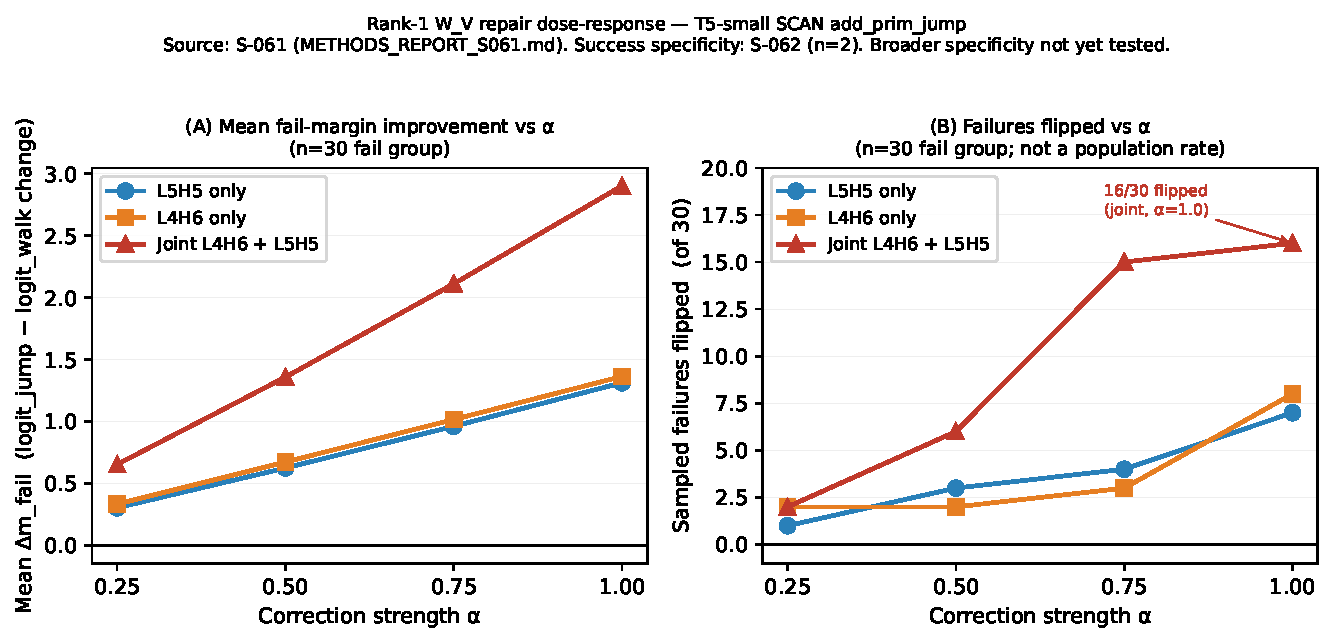
\includegraphics[width=\linewidth]{figures/fig06_rank1_repair_dose_response}
\caption{Rank-1 $W_V$ correction dose-response. T5-small fail group ($n=30$
substituted-walk examples, SEED=42). Three arms: L5H5 only, L4H6 only, joint
L4H6$+$L5H5. Response is monotonically linear across
$\alpha \in \{0.25, 0.50, 0.75, 1.00\}$.
At $\alpha=1.0$, joint correction shifts mean fail margin by $+2.90$ logit units
and flips 16/30 sampled failures.
This is a count in the sampled fail group --- not a population-level repair rate.
Success specificity: S-062, $n=2$; broader specificity against unrelated
\texttt{around}-commands not yet tested.}
\label{fig:dose-response}
\end{figure}

\subsection{Specificity Check and Limitations}

S-061 encountered a classifier bug in the success-group selection (a constraint copied
from the fail-group definition excluded all pure \texttt{jump around} success examples,
which contain no \texttt{I\_WALK} tokens in their targets).
S-062 corrected the classifier and evaluated H4 on the recoverable success group.

\paragraph{S-062 result.}
$n=2$ \texttt{jump around} success examples were available after the classifier fix.
Joint correction at $\alpha=1.0$ produced mean $\Delta m_\text{success}=+1.785$,
with 0/2 flip regressions (no working example broken) and 0/2 OOD cases (K2 clear).
The success-group margin improved, not degraded, under the correction.

\paragraph{Why this is expected, not a specificity result.}
The 2 success examples share the OOD \texttt{jump} encoder representation with the
fail group.
The correction redirects the same $W_V$ mapping of the same encoder direction;
that it improves the success examples is the mechanism working as designed.
It does not test whether the correction affects commands that do not invoke the
\texttt{jump} encoder direction at all.

\paragraph{H4 status: indeterminate.}
The degradation sub-test passed (0/2 flip regression, 0/2 OOD, K2 clear), confirming
the repair did not break the available correct examples.
The pre-registered broader specificity test --- non-\texttt{jump} \texttt{around}
commands (\texttt{walk around}, \texttt{run around}, \texttt{look around}) where the
OOD \texttt{jump} direction should not be active --- was not run.
H4 cannot be closed until that control is tested.
The honest claim is: the repair is confirmed non-degrading on the available success
sample; broader specificity is indeterminate.

\subsection{What This Does Not Establish}

\begin{itemize}
  \item \textbf{Universal repair of the jump$\to$walk substitution.}
    At $\alpha=1.0$, 14/30 sampled failures do not flip.
    The mean fail margin shifts from $-6.511$ to approximately $-3.6$ --- still
    pro-walk on average.
    A more complete repair would require additional correction strength, a different
    correction direction, or targeting additional heads beyond L4H6 and L5H5.

  \item \textbf{Broad specificity.}
    The correction was tested against 2 \texttt{jump around} success examples (S-062).
    Whether it affects commands that do not involve the \texttt{jump} encoder direction ---
    \texttt{walk around}, \texttt{run around}, \texttt{look around} --- is an open
    question.
    No regression testing on unrelated commands was performed.

  \item \textbf{$W_V$ failure as the only mechanism.}
    The rank-1 correction addresses the specific value-direction misalignment at L4H6
    and L5H5.
    The L6 cluster (L6H2, L5H6, L6H6, L6H5), which dominates the logit decomposition
    (S-059b) and shows negative ablation specificity (S-060), is not corrected.
    The repair does not re-decompose or eliminate the full near-cancellation structure
    identified in \S\ref{sec:explaining}.
    It improves the fail margin by redirecting the pro-walk signal at two heads, while
    leaving the larger compensatory L6 cluster unmodified.

  \item \textbf{Generalization beyond the sampled fail group.}
    All results are on the 30-example substituted-walk fail group (SEED=42).
    The 16/30 flip count is not a population-level repair rate for the full test set.
\end{itemize}
